\documentclass{standalone}
\usepackage{tikz}
\usetikzlibrary{patterns, positioning}


\begin{document}
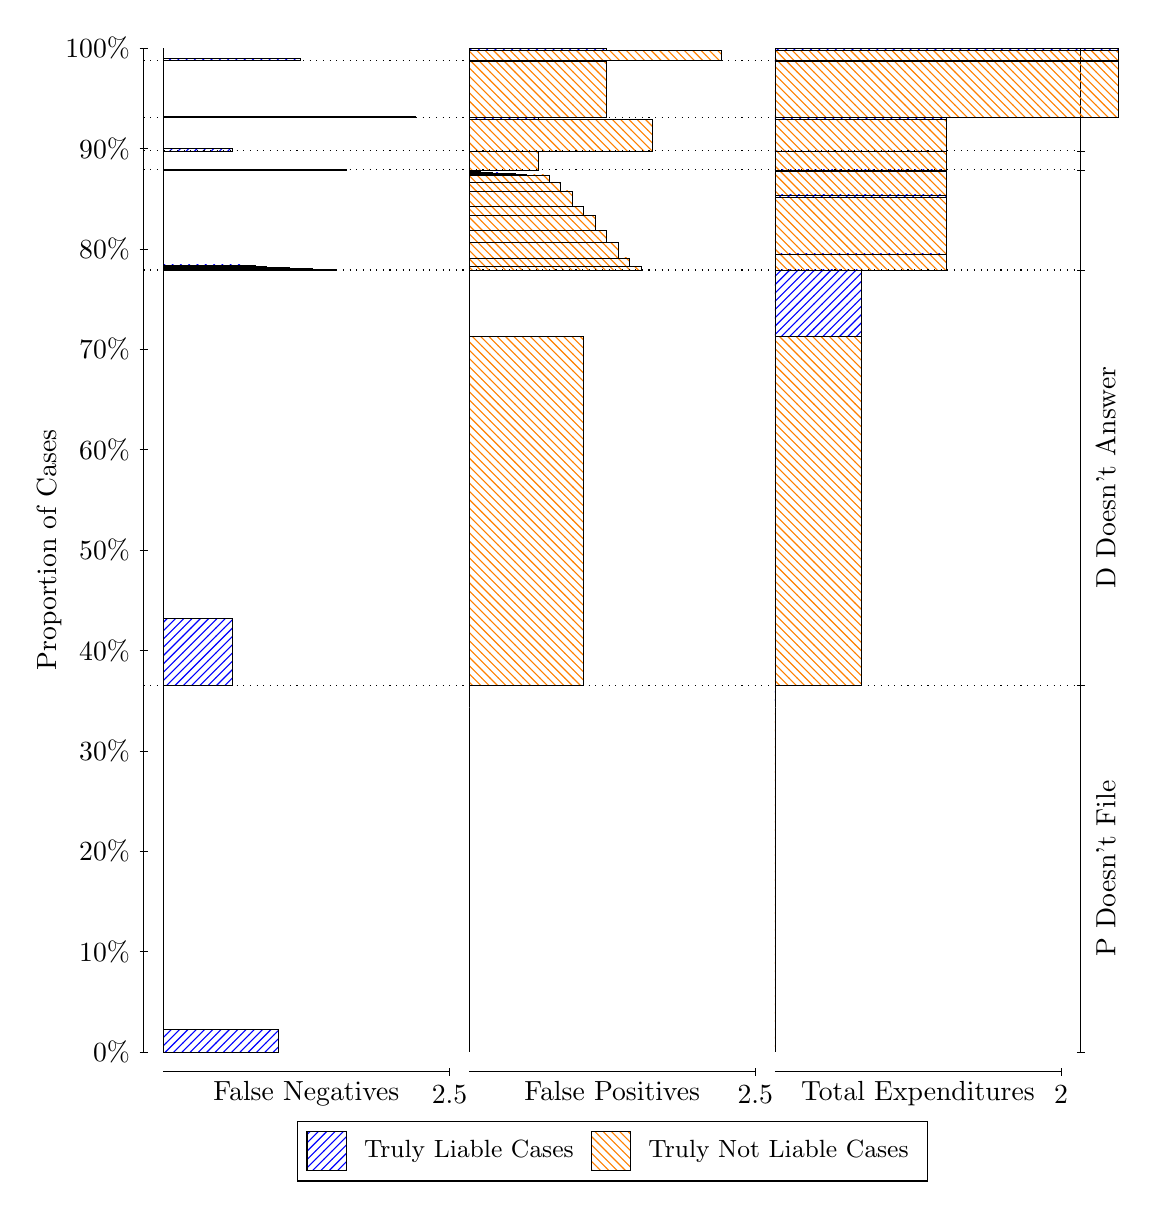
\begin{tikzpicture}
\draw[black, very thin] (1.5,1.75) -- (1.5,14.5);
\node[rotate=90, text=black, anchor=center] at (0.3, 8.125) {Proportion of Cases};
\draw[black, very thin] (1.45,1.75) -- (1.55,1.75);
\node[text=black, anchor=east] at (1.45, 1.75) {0\%};
\draw[black, very thin] (1.45,3.025) -- (1.55,3.025);
\node[text=black, anchor=east] at (1.45, 3.025) {10\%};
\draw[black, very thin] (1.45,4.3) -- (1.55,4.3);
\node[text=black, anchor=east] at (1.45, 4.3) {20\%};
\draw[black, very thin] (1.45,5.575) -- (1.55,5.575);
\node[text=black, anchor=east] at (1.45, 5.575) {30\%};
\draw[black, very thin] (1.45,6.85) -- (1.55,6.85);
\node[text=black, anchor=east] at (1.45, 6.85) {40\%};
\draw[black, very thin] (1.45,8.125) -- (1.55,8.125);
\node[text=black, anchor=east] at (1.45, 8.125) {50\%};
\draw[black, very thin] (1.45,9.4) -- (1.55,9.4);
\node[text=black, anchor=east] at (1.45, 9.4) {60\%};
\draw[black, very thin] (1.45,10.675) -- (1.55,10.675);
\node[text=black, anchor=east] at (1.45, 10.675) {70\%};
\draw[black, very thin] (1.45,11.95) -- (1.55,11.95);
\node[text=black, anchor=east] at (1.45, 11.95) {80\%};
\draw[black, very thin] (1.45,13.225) -- (1.55,13.225);
\node[text=black, anchor=east] at (1.45, 13.225) {90\%};
\draw[black, very thin] (1.45,14.5) -- (1.55,14.5);
\node[text=black, anchor=east] at (1.45, 14.5) {100\%};

\draw[black, very thin] (13.4,1.75) -- (13.4,14.5);
\draw[black, very thin] (13.35,1.75) -- (13.45,1.75);
\node[anchor=west] at (13.35, 1.75) {};
\draw[black, very thin] (13.35,6.4093) -- (13.45,6.4093);
\node[anchor=west] at (13.35, 6.4093) {};
\draw[black, very thin] (13.35,11.681) -- (13.45,11.681);
\node[anchor=west] at (13.35, 11.681) {};
\draw[black, very thin] (13.35,12.953) -- (13.45,12.953);
\node[anchor=west] at (13.35, 12.953) {};
\draw[black, very thin] (13.35,13.195) -- (13.45,13.195);
\node[anchor=west] at (13.35, 13.195) {};
\draw[black, very thin] (13.35,13.62) -- (13.45,13.62);
\node[anchor=west] at (13.35, 13.62) {};
\draw[black, very thin] (13.35,14.343) -- (13.45,14.343);
\node[anchor=west] at (13.35, 14.343) {};
\draw[black, very thin] (13.35,14.5) -- (13.45,14.5);
\node[anchor=west] at (13.35, 14.5) {};

\draw[black, very thin, pattern color=blue, pattern=north east lines] (1.75,1.75) rectangle (3.2033,2.0374);
\draw[black, very thin, pattern color=orange, pattern=north west lines] (1.75,2.0374) rectangle (1.75,6.4093);
\draw[black, very thin, pattern color=blue, pattern=north east lines] (1.75,6.4093) rectangle (2.622,7.2521);
\draw[black, very thin, pattern color=orange, pattern=north west lines] (1.75,7.2521) rectangle (1.75,11.681);
\draw[black, very thin, pattern color=blue, pattern=north east lines] (1.75,11.681) rectangle (3.93,11.686);
\draw[black, very thin, pattern color=blue, pattern=north east lines] (1.75,11.686) rectangle (3.7847,11.691);
\draw[black, very thin, pattern color=blue, pattern=north east lines] (1.75,11.691) rectangle (3.6393,11.699);
\draw[black, very thin, pattern color=blue, pattern=north east lines] (1.75,11.699) rectangle (3.494,11.705);
\draw[black, very thin, pattern color=blue, pattern=north east lines] (1.75,11.705) rectangle (3.3487,11.714);
\draw[black, very thin, pattern color=blue, pattern=north east lines] (1.75,11.714) rectangle (3.2033,11.719);
\draw[black, very thin, pattern color=blue, pattern=north east lines] (1.75,11.719) rectangle (3.058,11.731);
\draw[black, very thin, pattern color=blue, pattern=north east lines] (1.75,11.731) rectangle (2.9127,11.739);
\draw[black, very thin, pattern color=blue, pattern=north east lines] (1.75,11.739) rectangle (2.7673,11.745);
\draw[black, very thin, pattern color=orange, pattern=north west lines] (1.75,11.745) rectangle (1.75,12.953);
\draw[black, very thin, pattern color=blue, pattern=north east lines] (1.75,12.953) rectangle (4.0753,12.961);
\draw[black, very thin, pattern color=orange, pattern=north west lines] (1.75,12.961) rectangle (1.75,13.195);
\draw[black, very thin, pattern color=blue, pattern=north east lines] (1.75,13.195) rectangle (2.622,13.227);
\draw[black, very thin, pattern color=orange, pattern=north west lines] (1.75,13.227) rectangle (1.75,13.62);
\draw[black, very thin, pattern color=blue, pattern=north east lines] (1.75,13.62) rectangle (4.9473,13.635);
\draw[black, very thin, pattern color=orange, pattern=north west lines] (1.75,13.635) rectangle (1.75,14.343);
\draw[black, very thin, pattern color=blue, pattern=north east lines] (1.75,14.343) rectangle (3.494,14.37);
\draw[black, very thin, pattern color=orange, pattern=north west lines] (1.75,14.37) rectangle (1.75,14.5);
\draw[black, very thin, pattern color=orange, pattern=north west lines] (5.6333,1.75) rectangle (5.6333,6.1219);
\draw[black, very thin, pattern color=blue, pattern=north east lines] (5.6333,6.1219) rectangle (5.6333,6.4093);
\draw[black, very thin, pattern color=orange, pattern=north west lines] (5.6333,6.4093) rectangle (7.0867,10.838);
\draw[black, very thin, pattern color=blue, pattern=north east lines] (5.6333,10.838) rectangle (5.6333,11.681);
\draw[black, very thin, pattern color=orange, pattern=north west lines] (5.6333,11.681) rectangle (7.8133,11.73);
\draw[black, very thin, pattern color=orange, pattern=north west lines] (5.6333,11.73) rectangle (7.668,11.835);
\draw[black, very thin, pattern color=orange, pattern=north west lines] (5.6333,11.835) rectangle (7.5227,12.029);
\draw[black, very thin, pattern color=orange, pattern=north west lines] (5.6333,12.029) rectangle (7.3773,12.181);
\draw[black, very thin, pattern color=orange, pattern=north west lines] (5.6333,12.181) rectangle (7.232,12.377);
\draw[black, very thin, pattern color=orange, pattern=north west lines] (5.6333,12.377) rectangle (7.0867,12.485);
\draw[black, very thin, pattern color=orange, pattern=north west lines] (5.6333,12.485) rectangle (6.9413,12.687);
\draw[black, very thin, pattern color=orange, pattern=north west lines] (5.6333,12.687) rectangle (6.796,12.796);
\draw[black, very thin, pattern color=orange, pattern=north west lines] (5.6333,12.796) rectangle (6.6507,12.889);
\draw[black, very thin, pattern color=blue, pattern=north east lines] (5.6333,12.889) rectangle (6.36,12.895);
\draw[black, very thin, pattern color=blue, pattern=north east lines] (5.6333,12.895) rectangle (6.2147,12.904);
\draw[black, very thin, pattern color=blue, pattern=north east lines] (5.6333,12.904) rectangle (6.0693,12.915);
\draw[black, very thin, pattern color=blue, pattern=north east lines] (5.6333,12.915) rectangle (5.924,12.92);
\draw[black, very thin, pattern color=blue, pattern=north east lines] (5.6333,12.92) rectangle (5.7787,12.929);
\draw[black, very thin, pattern color=blue, pattern=north east lines] (5.6333,12.929) rectangle (5.6333,12.953);
\draw[black, very thin, pattern color=orange, pattern=north west lines] (5.6333,12.953) rectangle (6.5053,13.188);
\draw[black, very thin, pattern color=blue, pattern=north east lines] (5.6333,13.188) rectangle (5.6333,13.195);
\draw[black, very thin, pattern color=orange, pattern=north west lines] (5.6333,13.195) rectangle (7.9587,13.589);
\draw[black, very thin, pattern color=blue, pattern=north east lines] (5.6333,13.589) rectangle (6.5053,13.62);
\draw[black, very thin, pattern color=orange, pattern=north west lines] (5.6333,13.62) rectangle (7.3773,14.328);
\draw[black, very thin, pattern color=blue, pattern=north east lines] (5.6333,14.328) rectangle (5.924,14.343);
\draw[black, very thin, pattern color=orange, pattern=north west lines] (5.6333,14.343) rectangle (8.8307,14.473);
\draw[black, very thin, pattern color=blue, pattern=north east lines] (5.6333,14.473) rectangle (7.3773,14.5);
\draw[black, very thin, pattern color=orange, pattern=north west lines] (9.5167,1.75) rectangle (9.5167,6.1219);
\draw[black, very thin, pattern color=blue, pattern=north east lines] (9.5167,6.1219) rectangle (9.5167,6.4093);
\draw[black, very thin, pattern color=orange, pattern=north west lines] (9.5167,6.4093) rectangle (10.607,10.838);
\draw[black, very thin, pattern color=blue, pattern=north east lines] (9.5167,10.838) rectangle (10.607,11.681);
\draw[black, very thin, pattern color=orange, pattern=north west lines] (9.5167,11.681) rectangle (11.697,11.877);
\draw[black, very thin, pattern color=blue, pattern=north east lines] (9.5167,11.877) rectangle (11.697,11.886);
\draw[black, very thin, pattern color=orange, pattern=north west lines] (9.5167,11.886) rectangle (11.697,12.599);
\draw[black, very thin, pattern color=blue, pattern=north east lines] (9.5167,12.599) rectangle (11.697,12.635);
\draw[black, very thin, pattern color=orange, pattern=north west lines] (9.5167,12.635) rectangle (11.697,12.934);
\draw[black, very thin, pattern color=blue, pattern=north east lines] (9.5167,12.934) rectangle (11.697,12.953);
\draw[black, very thin, pattern color=orange, pattern=north west lines] (9.5167,12.953) rectangle (11.697,13.188);
\draw[black, very thin, pattern color=blue, pattern=north east lines] (9.5167,13.188) rectangle (11.697,13.195);
\draw[black, very thin, pattern color=orange, pattern=north west lines] (9.5167,13.195) rectangle (11.697,13.589);
\draw[black, very thin, pattern color=blue, pattern=north east lines] (9.5167,13.589) rectangle (11.697,13.62);
\draw[black, very thin, pattern color=orange, pattern=north west lines] (9.5167,13.62) rectangle (13.877,14.328);
\draw[black, very thin, pattern color=blue, pattern=north east lines] (9.5167,14.328) rectangle (13.877,14.343);
\draw[black, very thin, pattern color=orange, pattern=north west lines] (9.5167,14.343) rectangle (13.877,14.473);
\draw[black, very thin, pattern color=blue, pattern=north east lines] (9.5167,14.473) rectangle (13.877,14.5);
\draw[black, dotted] (1.5,6.4093) -- (13.4,6.4093);
\draw[black, dotted] (1.5,11.681) -- (13.4,11.681);
\draw[black, dotted] (1.5,12.953) -- (13.4,12.953);
\draw[black, dotted] (1.5,13.195) -- (13.4,13.195);
\draw[black, dotted] (1.5,13.62) -- (13.4,13.62);
\draw[black, dotted] (1.5,14.343) -- (13.4,14.343);
\draw[black, very thin] (1.75,1.5) -- (5.3833,1.5);
\node[text=black, anchor=north] at (3.5667, 1.5) {False Negatives};
\draw[black, very thin] (5.3833,1.45) -- (5.3833,1.55);
\node[text=black, anchor=north] at (5.3833, 1.45) {2.5};

\draw[black, very thin] (5.6333,1.5) -- (9.2667,1.5);
\node[text=black, anchor=north] at (7.45, 1.5) {False Positives};
\draw[black, very thin] (9.2667,1.45) -- (9.2667,1.55);
\node[text=black, anchor=north] at (9.2667, 1.45) {2.5};

\draw[black, very thin] (9.5167,1.5) -- (13.15,1.5);
\node[text=black, anchor=north] at (11.333, 1.5) {Total Expenditures};
\draw[black, very thin] (13.15,1.45) -- (13.15,1.55);
\node[text=black, anchor=north] at (13.15, 1.45) {2};

\node[text=black, centered, rotate=90] at (13.72, 4.0797) {P Doesn't File};
\node[text=black, centered, rotate=90] at (13.72, 9.0451) {D Doesn't Answer};






\draw (7.449999999999999,1.5) node[draw=none] (baseCoordinate) {};
\begin{scope}[align=center]
        \matrix[scale=0.5, draw=black, below=0.5cm of baseCoordinate, nodes={draw}, column sep=0.1cm]{
            \node[rectangle, draw, minimum width=0.5cm, minimum height=0.5cm, pattern color=blue, pattern=north east lines] {}; &
            \node[draw=none, font=\small, text=black] (B) {Truly Liable Cases}; &
            \node[rectangle, draw, minimum width=0.5cm, minimum height=0.5cm, pattern color=orange, pattern=north west lines] {}; &
            \node[draw=none, font=\small, text=black] (B) {Truly Not Liable Cases}; \\
            };
\end{scope}

\end{tikzpicture}
\end{document}